
\documentclass[tikz,letterpaper,twocolumn,10pt]{article}
\usepackage{tikz}
\usetikzlibrary{positioning, arrows.meta}
\usepackage{graphicx}
\usepackage{usenix-2020-09}

% to be able to draw some self-contained figs
\usepackage{tikz}
\usepackage{amsmath}

% inlined bib file
\usepackage{filecontents}


%-------------------------------------------------------------------------------
\begin{document}
%-------------------------------------------------------------------------------

%don't want date printed
\date{}

% make title bold and 14 pt font (Latex default is non-bold, 16 pt)
\title{\Large \bf IP Shuffle:\\
  Random IP Address Assignment for Network Interfaces}

%for single author (just remove % characters)
\author{
{\rm Hunter Thompson}\\
Eastern Washington University
\and
{\rm Chelsea Edwards}\\
Eastern Washington University
% copy the following lines to add more authors
% \and
% {\rm Name}\\
%Name Institution
} % end author

\maketitle

%-------------------------------------------------------------------------------
\begin{abstract}
%-------------------------------------------------------------------------------
This paper introduces a Bash script designed to dynamically assign a random IP address to a computer's network interface. The script generates a random IP address within a specified range, checks its availability, and ensures proper configuration. It achieves efficient and reliable IP address assignment through distinct functions for IP address generation, availability verification, network configuration validation, and gateway reachability testing. The IP-shuffle script provides a practical solution for scenarios that require dynamic IP address allocation and streamlining network management processes. Its robustness is further enhanced by comprehensive error handling and compatibility with Linux and BSD systems.
\end{abstract}


%-------------------------------------------------------------------------------
\section{Introduction}
%-------------------------------------------------------------------------------
The MTD technique that were working towards is IP shuffling, to make 
lateral movement reconnaissance much more difficult. This strategy 
involves the dynamic changing of IP addresses of systems on a network. 
In our model, we have a private subnet containing 3 virtual machines. 
These machines perform IP address rotation, executing erratic or periodic
shifts across a 254 different IP addresses. Furthermore, our diagram 
illustrates an instance where one of these computers, denoted as Computer 1,
has been compromised. By continuously changing IP addresses in an 
unpredictable manner, IP shuffling impedes the reconnaissance efforts of 
attackers, making it difficult for them to pinpoint and exploit vulnerabilities.
The diagram delineates the intricate architecture of our network infrastructure, 
illustrating the hierarchical arrangement of networks, subnets, and their 
corresponding topological relationships. Within this schematic representation, 
the affected computer is depicted, providing a visual reference to its 
position within the broader network.  


%-------------------------------------------------------------------------------
\section{Threat Background}
%-------------------------------------------------------------------------------
Our threat model concerns the scenario in which a system is attacked. Specifically, we focus on the scenario depicted in the diagram, where 
three interconnected computers form a network, with one of these computers compromised. Within this context, our threat model revolves around 
an attacker who has successfully gained access to one of the systems, as illustrated in the diagram. Once inside the network, the attacker's 
assumed objective is to scan other systems to identify vulnerabilities for lateral movement. The provided script, named "ip-shuffle," plays a crucial 
role in this threat scenario, as it allows for the dynamic assignment of random IP addresses to network interfaces. The attackers capabilities 
could possibly be but not limited to exploitation skills because of the knowledge of common vulnerabilities, network reconnaissance
by scanning the network to identify other vulernabilities, and persistence. The "ip-shuffle" with the random timing and frequency of IP address changes
makes it harder for attackers to predict when the changes will occur for the attackers assumed abilites. It also makes it difficult to map out the 
network accurately, this can confuse attackers and make it harder for them to identify and target vulnerable systems.

This proactive approach aligns with the broader goals of MT techniques, which prioritize enhancing system resilience against cyber 
threats. While certain MT techniques like Address Space Layout Randomization (ASLR) have achieved widespread adoption in modern operating 
systems, implementing IP shuffling provides an additional layer of defense that can complement existing security measures. By adopting IP 
shuffling and other MT techniques, organizations can strengthen their overall security posture and mitigate the impact of cyber threats.
For instance, dynamically changing IP addresses, randomizing memory layouts, and employing temporary encryption for memory contents fall 
within the spectrum of MT techniques~\cite{okhravi2013finding}.

%-------------------------------------------------------------------------------
\section{System Design}

The IP-shuffle script offers a systematic approach to dynamic IP address assignment for network interfaces in Linux and FreeBSD environments. Built around Bash scripting, it seamlessly orchestrates the IP address allocation process. By default, the program runs every 3 minutes, based on the provided cronjob. During execution, the script dynamically configures the IP address, gateway, network interface details, and other parameters, providing a flexible framework for network configuration. Through dedicated functions such as
\begin{verbatim}
generate_random_ip (), 
check_ip_availability(), 
and validate_network_config(), 
\end{verbatim}
the script ensures that the assigned IP addresses are compatible with the network infrastructure. It also incorporates error-trapping mechanisms and support for common Unix signals to enhance reliability and resilience, safeguarding against potential errors or interruptions. The script's flexibility is maintained through adherence to modular design principles, allowing seamless adaptation to diverse network configurations and environments. However, since the IP addresses are not persistent after a reboot for DHCP-configured machines, the script includes functions like \texttt{reset\_network()} for error recovery. The IP-shuffle script encapsulates a robust solution for automating network interface configuration tasks, embodying a sophisticated yet accessible approach to dynamic IP address management.

\label{sec:figs}
%-------------------------------------------------------------------------------
%---------------------------


\begin{figure}
 \caption{Network Topology Diagram}
  \centering
   \includegraphics[width=0.5\textwidth]{diagram.png}
\end{figure}

%% %---------------------------
 





%-------------------------------------------------------------------------------
%-------------------------------------------------------------------------------
\section{Evaluation}

To evaluate the effectiveness of our IP shuffling script, we'll be adding an extra system to the virtual network with a static IP address of \texttt{192.168.1.10}. We'll be setting up an OPNsense instance as the default gateway for all virtual machines. This instance will be assigned the IP address \texttt{192.168.1.1}, and it will act as a simulated router that provides the DHCP service. As shown in Figure 1, there will be two Ubuntu Linux machines and one instance of FreeBSD. Each machine will receive an IP address on initial startup starting at \texttt{192.168.1.100}, assigned by OPNsense. We'll give each system 6 minutes after startup to begin changing its IP address, after which we'll use an arp-scan to obtain the following output:
\begin{verbatim}
192.168.1.1     00:1c:42:c1:e4:da       (Unknown)
192.168.1.103   00:1c:42:c6:34:d1       (Unknown)
192.168.1.200   00:1c:42:98:99:4d       (Unknown)
192.168.1.236   00:1c:42:76:c0:7e       (Unknown)
\end{verbatim}
We can observe that the IP addresses, with the exception of the OPNsense instance, have been altered from their initially assigned addresses through DHCP. To check if the systems have changed their IPs once more, let's wait for another six minutes and then conduct another ARP scan. Here are the results of the said scan:
\begin{verbatim}
192.168.1.1     00:1c:42:c1:e4:da       (Unknown)
192.168.1.71    00:1c:42:76:c0:7e       (Unknown)
192.168.1.199   00:1c:42:c6:34:d1       (Unknown)
192.168.1.211   00:1c:42:98:99:4d       (Unknown)
\end{verbatim}
Let's cross-check the modified IP addresses with their respective MAC addresses for a clearer understanding of their altered IPs.

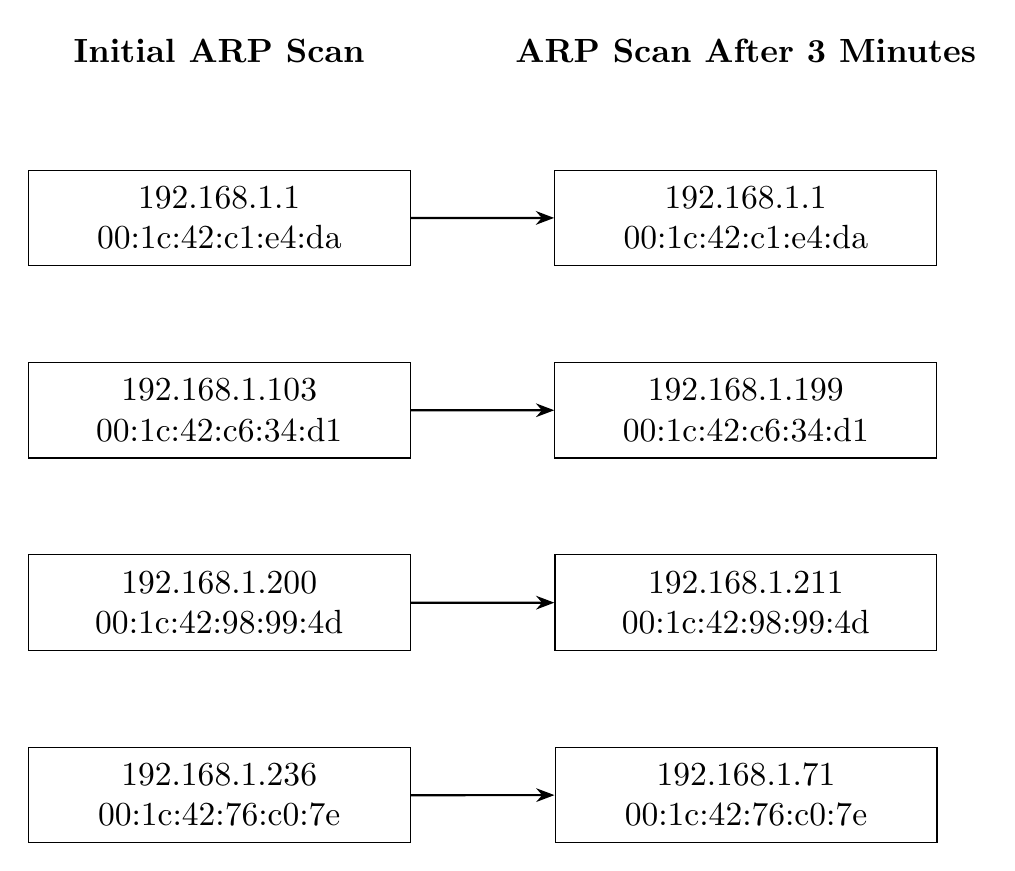
\begin{tikzpicture}[ 
  node distance=1cm and 1.5cm,
  box/.style={rectangle, draw, minimum height=1cm, minimum width=4cm, align=center},
  arrow/.style={-Stealth, thick},
  scale=\linewidth/10cm, transform shape
]

  % Original IP-MAC pairs
  \node[box] (old1) {192.168.1.1\\00:1c:42:c1:e4:da};
  \node[box, below=of old1] (old2) {192.168.1.103\\00:1c:42:c6:34:d1};
  \node[box, below=of old2] (old3) {192.168.1.200\\00:1c:42:98:99:4d};
  \node[box, below=of old3] (old4) {192.168.1.236\\00:1c:42:76:c0:7e};

  % New IP-MAC pairs
  \node[box, right=of old1] (new1) {192.168.1.1\\00:1c:42:c1:e4:da};
  \node[box, below=of new1] (new2) {192.168.1.199\\00:1c:42:c6:34:d1};
  \node[box, below=of new2] (new3) {192.168.1.211\\00:1c:42:98:99:4d};
  \node[box, below=of new3] (new4) {192.168.1.71\\00:1c:42:76:c0:7e};

  % Arrows showing changes
  \draw[arrow] (old1) -- (new1);
  \draw[arrow] (old2) -- (new2);
  \draw[arrow] (old3) -- (new3);
  \draw[arrow] (old4) -- (new4);

  % Labels
  \node[above=of old1] (labelOld) {\textbf{Initial ARP Scan}};
  \node[above=of new1] (labelNew) {\textbf{ARP Scan After 3 Minutes}};

\end{tikzpicture}

%-------------------------------------------------------------------------------
%-------------------------------------------------------------------------------
\section{Conclusion}

Moving Target Defense (MTD) is a "game-changing" theme in cybersecurity that involves creating mechanisms and strategies that are diverse, continually shifting, and changing over time to increase complexity and costs for attackers, limit the exposure of vulnerabilities, and increase system resiliency~\cite{cai2016introduction}.. The IP-shuffle script provides a robust solution for dynamically allocating random IP addresses to network interfaces, a critical component of network security strategies aimed at deterring potential attackers.
Leveraging Bash scripting, the IP-shuffle script offers functionalities for generating random IP addresses, checking their availability, and validating network configurations, ensuring efficient and reliable IP address assignment. It also incorporates error-handling capabilities and Unix signal responsiveness, enhancing reliability during execution and strengthening network resilience. Its modular design allows for easy adaptation to different network setups, making it a valuable tool for automating network interface configuration tasks.
The IP-shuffle script embodies the concept of IP shuffling, a technique designed to complicate attackers' reconnaissance efforts by constantly changing IP addresses unpredictably. By dynamically assigning random IP addresses, IP-shuffle enhances proactive defense strategies, increasing the difficulty for attackers to identify and exploit vulnerabilities.
%-------------------------------------------------------------------------------
\bibliographystyle{plain}
\bibliography{refs}

%%%%%%%%%%%%%%%%%%%%%%%%%%%%%%%%%%%%%%%%%%%%%%%%%%%%%%%%%%%%%%%%%%%%%%%%%%%%%%%%
\end{document}
%%%%%%%%%%%%%%%%%%%%%%%%%%%%%%%%%%%%%%%%%%%%%%%%%%%%%%%%%%%%%%%%%%%%%%%%%%%%%%%%

%%  LocalWords:  endnotes includegraphics fread ptr nobj noindent
%%  LocalWords:  pdflatex acks
